\documentclass[hyperref={pdftex,unicode}]{beamer}
\usepackage[T2A]{fontenc}
\usepackage[utf8]{inputenc}
\usepackage[russian]{babel}
\usepackage{amssymb,amsfonts,amsmath,mathtext}
\usepackage{cite,enumerate,float,indentfirst}
\usepackage{cmap}

\graphicspath{{images/}}

\usefonttheme{professionalfonts}
\usefonttheme[onlymath]{serif}
\setbeamerfont{institute}{size=\normalsize}
%\usepackage{times}
%%\setmainfont{Liberation Serif}

\usecolortheme{seagull}

\setbeamercolor{footline}{fg=gray}
\setbeamertemplate{footline}{
  \leavevmode%
  \hbox{%
  \begin{beamercolorbox}[wd=1\paperwidth,ht=2.25ex,dp=1ex,right]{}%
  Стр. \insertframenumber{} из \inserttotalframenumber \hspace*{2ex}
  \end{beamercolorbox}}%
  \vskip0pt%
}

\newcommand{\itemi}{\item[\checkmark]}

\title{Применение метода Пенлеве для исследования режимов работы асинхронных двигателей}

\author{
 Выступающие: П. С. Анашкевич, Р. И. Будный
}
\institute{
    Научный руководитель:  ~проф.,~д.ф.-м.н.~В. В.Цегельник \\
    \vspace{40pt}
}

\date{Минск, 2013}

\begin{document}

\begin{frame}

\vspace{40pt}
\maketitle

\end{frame}



\begin{frame}
\frametitle{Постановка задачи}

\begin{itemize}

\item{Произвести математическое описание работы АД\footnote{Асинхронный двигатель}}
\item{Исследовать АД на предмет наличия неустойчивых режимов работы}

\end{itemize}

\end{frame}



\begin{frame}

\frametitle{Асинхронный двигатель}

Асинхронный двигатель --- электрическая машина переменного тока, частота вращения ротора которой не равна частоте вращения магнитного поля, создаваемого током обмотки статора.

%%Про беличью клетку

\end{frame}


\begin{frame}
\frametitle{Асинхронный двигатель}

\begin{figure}[H]
  \center
  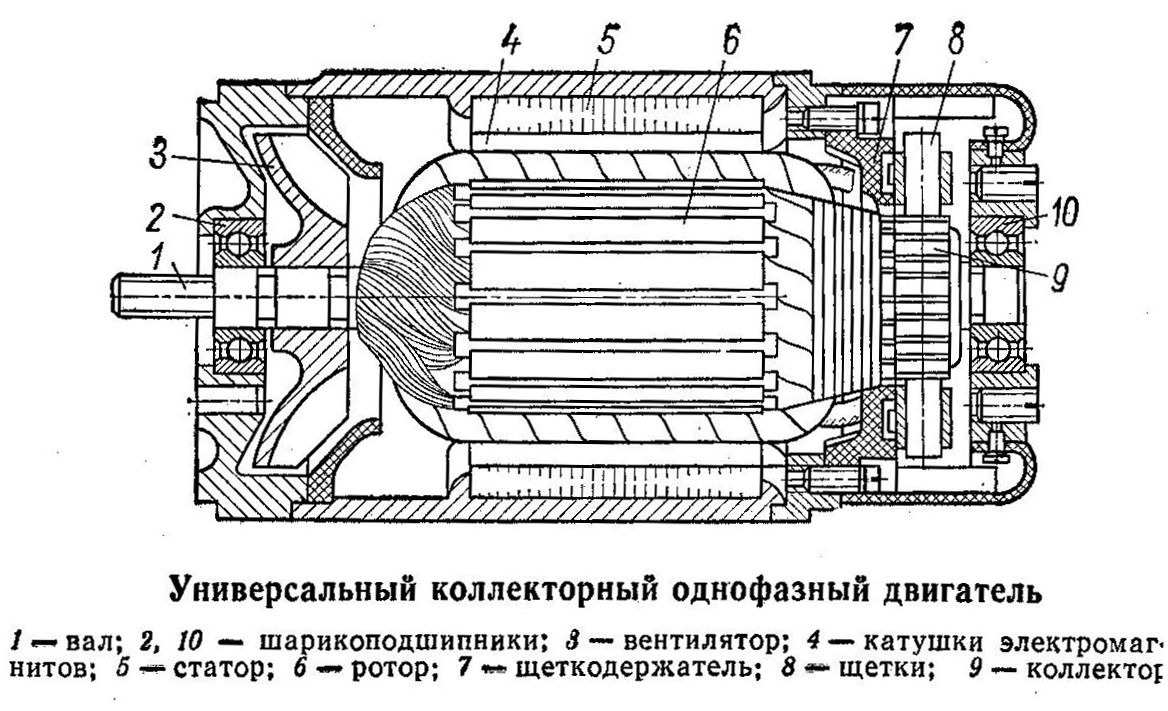
\includegraphics[width=0.8\linewidth]{construction}
\end{figure}

\end{frame}


\begin{frame}
\frametitle{Асинхронный двигатель}

\begin{figure}[H]
  \center
  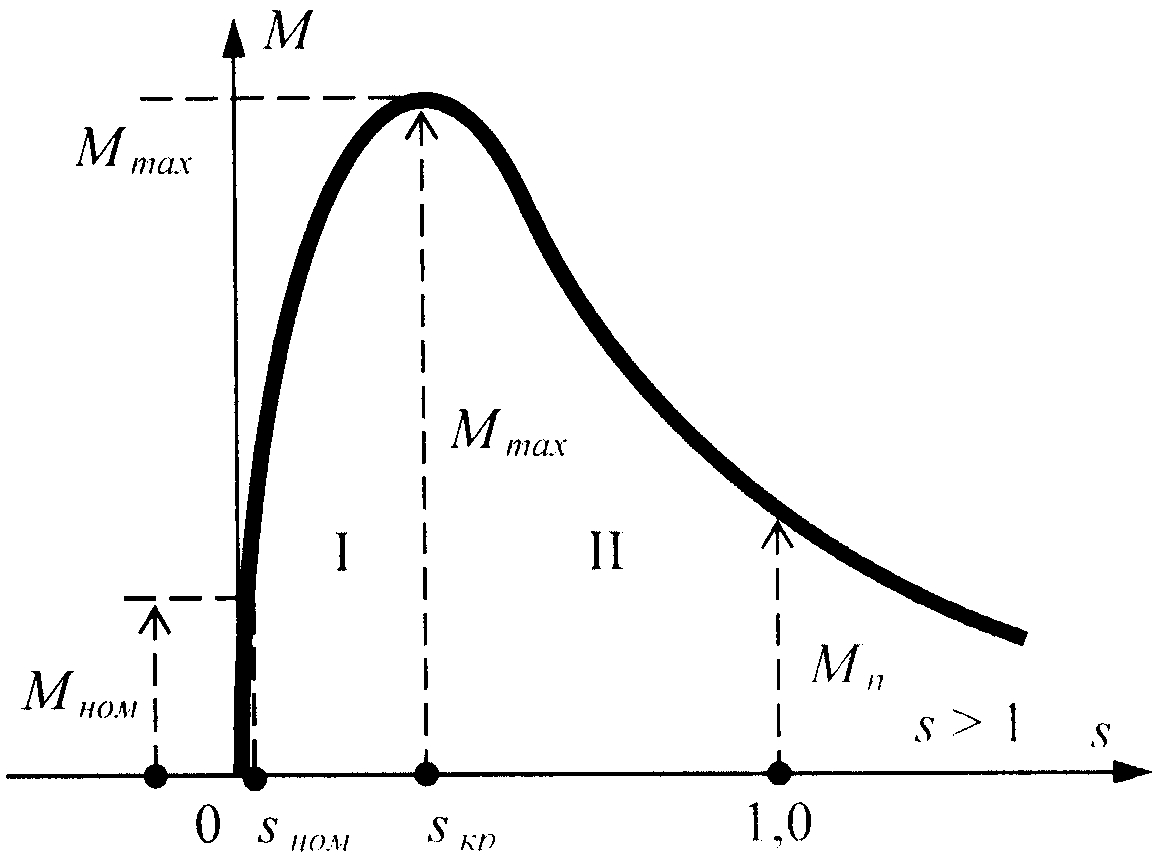
\includegraphics[width=0.6\linewidth]{zavisimost-1}
\end{figure}

\vspace{10pt}

\small{s -- скольжение: $ s = 1 - \dfrac{n}{n_c} $}	

\small{M -- крутящий момент}
	

\end{frame}




\begin{frame}
\frametitle{Поль Пенлеве (1863 -- 1933)}

\begin{figure}[H]
  \center
  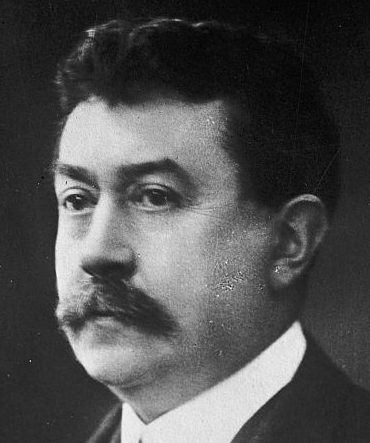
\includegraphics[width=0.4\linewidth]{penleve}
\end{figure}

\vspace{10pt}
Французский математик и политик. Один из создателей аналитической теории дифференциальных уравнений. Был дважды премьер-министром Третьей Республики.
\end{frame}


\begin{frame}

\frametitle{$\alpha $-метод Пенлеве}

Универсальный метод.

Основан на методе малого параметра Пуанкаре. 

Используется для анализа дифференциальных уравнений. 

\end{frame}


\begin{frame}
\frametitle{Модель}

\begin{figure}[H] 
  \begin{center}

  \begin{minipage}[h]{0.4\linewidth}

  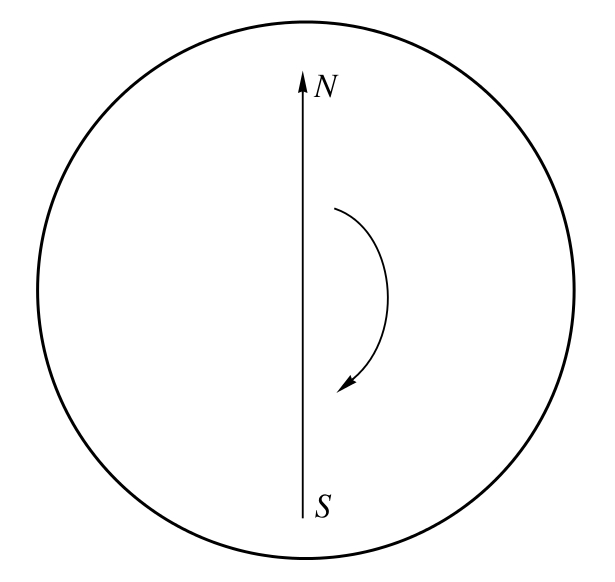
\includegraphics[width=1\linewidth]{magnitnoe_pole}

  \center{\small{Вращающееся \\ магнитное поле}}
  
  \end{minipage}
  \hfill   
  \begin{minipage}[h]{0.4\linewidth}
    
  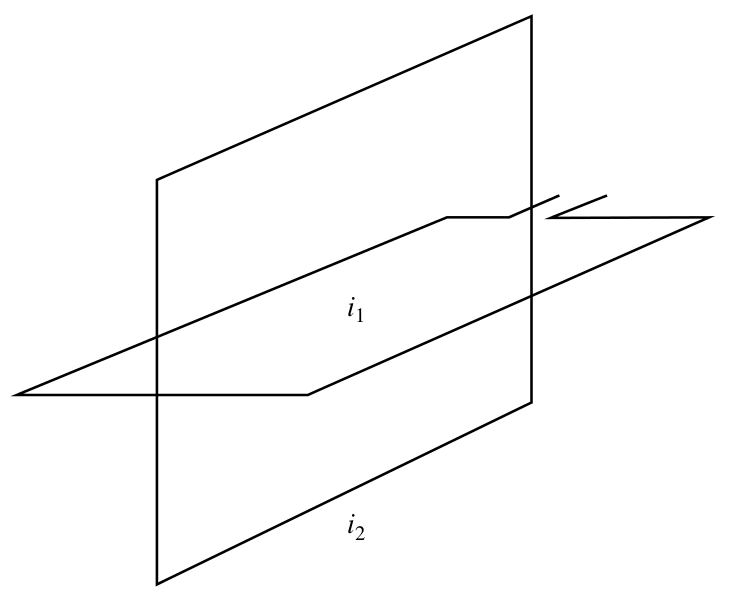
\includegraphics[width=1\linewidth]{obmotki}
  
  \center{\small{Схема обмоток}}
  \end{minipage}    
    
  \end{center}
\end{figure}


\end{frame}


\begin{frame}

\frametitle{Физическое описание}
$$
        \left\{
                \begin{aligned}
                        L \dfrac{di_1(t)}{dt} + Ri_1(t) = e + SB(\sin\theta(t)) \dot \theta (t), \\
                        L \dfrac{di_2(t)}{dt} + Ri_2(t) = e + SB(\cos\theta(t)) \dot \theta (t),
\\
  						I \ddot \theta = -\beta SB(i_1(t)\sin\theta + i_2(t)\cos\theta) - M.
                \end{aligned}
        \right.
$$

\vspace{20pt}

Сделаем замены: $ s = \dot \theta_1 = - \dot \theta, a = \dfrac{\beta(SB)^2}{IL}, c = \dfrac{R}{L}, $

\hspace{105pt} $ x = \dfrac{L}{SB} (i_1\cos\theta_1 + i_2\sin\theta_1),$

\vspace{5pt}

\hspace{105pt} $ y = \dfrac{L}{SB} (-i_1\sin\theta_1 + i_2\cos\theta_1).$

\end{frame}


\begin{frame}

\frametitle{Исходная система}

$$
        \left\{
                \begin{aligned}
                        \dot s &= ay + \gamma , \\
                        \dot y &= -cy -s -xs , \\
                        \dot x &= cx + ys .
                \end{aligned}
        \right. 
$$

\vspace{20pt}

Применим метод Пенлеве для отыскания решения системы относительно $ x, y, s $.

\end{frame}



\begin{frame}

\frametitle{Метод Пенлеве: шаг 1}

Пусть $ s = \dfrac{s_0}{\tau^k}, y = \dfrac{y_0}{\tau^l} , x = \dfrac{x_0}{\tau^m} $, 
\vspace{5pt}
где $ \tau = (t - t_0) $ -- произвольная постоянная:
$$    
         \left\{
                \begin{aligned}
                        -\dfrac{ks_0}{\tau^{k+1}} &= a \dfrac{y_0}{\tau^l} + \gamma , \\
                        -\dfrac{ly_0}{\tau^{l+1}} &= -c \dfrac{y_0}{\tau^l} - \dfrac{s_0}{\tau^k} - \dfrac{x_0}{\tau^m} \dfrac{s_0}{\tau^k} , \\
                        -\dfrac{mx_0}{\tau^{m+1}} &= -c \dfrac{x_0}{\tau^m} + \dfrac{y_0}{\tau^l} \dfrac{s_0}{\tau^k} .
                \end{aligned}
        \right.
$$

\vspace{20pt}

Учитывая, что $ k $, $ l $, $ m \in \textbf{Z} $, получим: $ m = 2, k = 1, l = 2 $.


\end{frame}



\begin{frame}

\frametitle{Метод Пенлеве: шаг 1}

$$
        \left\{
                \begin{aligned}
                        -\dfrac{s_0}{\tau^2} &= a \dfrac{y_0}{\tau^2} + \gamma, \\
                        -\dfrac{2y_0}{\tau^3} &= -c \dfrac{y_0}{\tau^2} - \dfrac{s_0}{\tau} - \dfrac{x_0 s_0}{\tau^3}, \\
                        -\dfrac{2x_0}{\tau^{3}} &= -c \dfrac{x_0}{\tau^2} + \dfrac{y_0 s_0}{\tau^3}.
                \end{aligned}
        \right.
$$

\vspace{20pt}

Приравняв коэффициенты при одинаковых степенях $ \tau $, получим:

\vspace{10pt}

\begin{minipage}[h!]{0.4\linewidth}
$$
\left\{
\begin{aligned}
  x_0 &= - \dfrac{2}{a}, \\
  y_0 &= -\dfrac{2i}{a}, \\
  s_0 &= 2i, \\
\end{aligned}
\right.
$$
\end{minipage}
\hfill
либо
\hfill
\begin{minipage}[h!]{0.4\linewidth}
$$
\left\{
\begin{aligned}
  x_0 &= - \dfrac{2}{a}, \\
  y_0 &= \dfrac{2i}{a}, \\
  s_0 &= - 2i. 
\end{aligned}
\right.
$$
\end{minipage}


\end{frame}

\begin{frame}

\frametitle{Метод Пенлеве: шаг 2}

Сделаем подстановку в виде
 
\vspace{10pt}
$ 
s = \dfrac{s_0}{\tau} + \alpha \tau^{r-1},
y = \dfrac{y_0}{\tau^2} + \beta \tau^{r-2},                         x = \dfrac{x_0}{\tau^2} + \theta \tau^{r-2} $:

\tiny{
$$
        \left\{
                \begin{aligned}
                        -\dfrac{s_0}{\tau^{2}} + \alpha (r-1) \tau^{r-2} &= a \left( \dfrac{y_0}{\tau^2} + \beta \tau^{r-2} \right) + \gamma , \\
                        -\dfrac{2y_0}{\tau^{3}} + \beta (r-2) \tau^{r-3} &= -c \left( \dfrac{y_0}{\tau^2} + \beta \tau^{r-2} \right) - \left( \dfrac{s_0}{\tau} + \alpha \tau^{r-1} \right) - \left( \dfrac{x_0}{\tau^2} + \theta \tau^{r-2} \right) \left( \dfrac{s_0}{\tau} + \alpha \tau^{r-1} \right) , \\
                        -\dfrac{2x_0}{\tau^{3}} + \theta (r-2) \tau^{r-3} &= -c \left( \dfrac{x_0}{\tau^2} + \theta \tau^{r-2} \right) + \left( \dfrac{y_0}{\tau^2} + \beta \tau^{r-2} \right) \left( \dfrac{s_0}{\tau} + \alpha \tau^{r-1} \right) .
                \end{aligned}
        \right.
$$
}

\end{frame}



\begin{frame}

\frametitle{Метод Пенлеве: шаг 2}

Составим матрицу из коэффициентов при $ \alpha $, $ \beta $, $ \theta $:

\vspace{10pt}

$$
\left(
                \begin{array}{ccc}
                        r-1 & -a & 0 \\
                        x_0 & r-2 & s_0 \\
                        -y_0 & -s_0 & r-2 \\
                \end{array}
\right)
$$

\vspace{20pt}

Приравняв определитель матрицы к нулю, получим:

\center{$ r_1 = - 1, r_2 = 2, r_3 = 4 $.}

\end{frame}



\begin{frame}

\frametitle{Метод Пенлеве: шаг 3}

Будем искать решение системы в виде:

$$
        \left\{
                \begin{aligned}
                        s &= \dfrac{s_{-1}}{\tau} + s_0 + s_1\tau + s_2\tau^2 + s_3\tau^3 + \ldots ~,  \\
                        y &= \dfrac{y_{-2}}{\tau^2} + \dfrac{y_{-1}}{\tau} + y_0 + y_1\tau + y_2\tau^2 + y_3\tau^3 + \ldots ~, \\
                        x &= \dfrac{x_{-2}}{\tau^2} + \dfrac{x_{-1}}{\tau} + x_0 + x_1\tau + x_2\tau^2 + x_3\tau^3 + \ldots ~.
                \end{aligned}
        \right.
$$

\vspace{20pt}

Подставим его в систему, приравняем коэффициенты при одинаковых степенях $ \tau $, сгруппируем по степеням $ r $.


\end{frame}



\begin{frame}

\frametitle{Анализ решения}
\begin{minipage}[H]{0.4\linewidth}

$$
r = 0:
\left\{
	\begin{aligned}
		s_{-1} &= -2 \\
		y_{-2} &= \dfrac{2}{a} \\
		x_{-2} &= \dfrac{2}{a}
	\end{aligned}
\right.
$$

\end{minipage}
\hfill
\begin{minipage}[H]{0.4\linewidth}

$$
r = 1:
\left\{
	\begin{aligned}
		s_{0} &= \dfrac{c}{3} \\
		y_{-1} &= 0 \\
		x_{-1} &= \dfrac{4c}{3a}
	\end{aligned}
\right.
$$

\end{minipage}

\vspace{20pt}

$$
r = 2:
\left\{
	\begin{aligned}
		y_{0} &- \text{произвольный} \\
		s_{1} &= ay_0 + \dfrac{2c^2}{3} \\
		x_{0} &= \dfrac{8c^2}{9a} - 1 + y_0
	\end{aligned}
\right.
$$

\end{frame}



\begin{frame}

\frametitle{Анализ решения}

$$
\begin{aligned}
r = 3 &:
\left\{
	\begin{aligned}
		y_1 &= -\dfrac{20c^3}{27} - cy_0 + \dfrac{c}{2} \\
		x_1 &= -\dfrac{4c^3}{27a} + \dfrac{cy_0}{3} + \dfrac{c}{2} \\
		s_2 &= -\dfrac{10c^3}{27} - \dfrac{cay_0}{2} + \dfrac{ca}{4}
	\end{aligned}
\right.
\\
r = 4 &: 
\left\{
	\begin{aligned}
		x_2 &= -\dfrac{50c^4}{243} + \dfrac{14c^4}{243a} + \dfrac{c^2}{18} + \dfrac{ay^2_0}{2}\\
		y_2 &= \dfrac{10c^4}{81} + \dfrac{2c^4}{81a} - \dfrac{c^2}{3} \\
		s_3 &= \dfrac{10ac^4}{243} + \dfrac{2c^4}{243} - \dfrac{ac^2}{9}
	\end{aligned}
\right.
\end{aligned}
$$

\end{frame}



\begin{frame}

\frametitle{Анализ решения}

\begin{itemize}

\item
Степени $ \tau $, при которых следует искать произвольные постоянные, равны значениям r, полученным в шаге 2: 
\begin{center}
$ r = -1, 2, 4. $ 
\end{center}

\item
Действительно, среди полученных коэффициентов имеется одна произвольная постоянная --- $ y_0 $ при $ r = 2 $.

\item
Таким образом, мы имеем две произвольные постоянные: $ t_0 $ и $ y_0 $.

\end{itemize}
\end{frame}


\begin{frame}

\frametitle{Выводы}

\begin{itemize}

\item
Для того, чтобы утверждать, что модель АД устойчива при любых $x, y, s, \tau $, необходимо найти 3 произвольные постоянные при $ \tau^{r_i} $.

\item
Мы нашли две: $ t_0 $ (из условия) и $ y_0 $.

\item
Это говорит о существовании неустойчивых режимов работы (в математическом смысле).

\end{itemize}


\end{frame}


\begin{frame}
\begin{center}

Спасибо за внимание!

\end{center}
\end{frame}


\begin{frame}
\frametitle{Литература}

\begin{enumerate}
\item{Леонов Г. А.: Фазовая синхронизация. Теория и приложения.}
\item{Кудряшов Н. А.: Аналитическая теория нелинейных дифференциальных уравнений.}

\item{http://model.exponenta.ru/electro/0080.htm}
\item{http://ru.wikipedia.org}

\end{enumerate}

\end{frame}

\end{document} 
